\documentclass{article}
\usepackage{times}
\usepackage[nohead,bottom=3cm,top=2cm,a4paper]{geometry}
\usepackage[table]{xcolor}
\usepackage{graphicx}
\usepackage[nswissgerman]{babel}
\usepackage{listings}
\usepackage{blindtext}
\usepackage{enumitem}
\usepackage{lipsum}
\usepackage{tikz}
\usepackage{hyperref}
\usepackage{float}
\usepackage{fontawesome}
\usepackage{mathtools}
\usetikzlibrary{positioning}
\usepackage{amssymb,amsmath,amsthm}
\graphicspath{ {./results/} }
\usetikzlibrary{shadows,matrix} % Shadows for nodes
\usetikzlibrary{arrows.meta}
\title{Report aus dem Projekt sensor Cube}
\newlength\mylength
\setlength\mylength{\dimexpr.42\columnwidth-2\tabcolsep-0.42\arrayrulewidth\relax}
\usepackage[section]{placeins}
\def\l@subsection{\@tocline{2}{0pt}{2.5pc}{5pc}{}}	
\definecolor{Gray}{gray}{0.9}
\makeatletter
\renewcommand*\l@section{\@dottedtocline{1}{1.5em}{2.3em}}
\makeatother
\usepackage{varioref}

\author{von Ugur Turhal, Berkan Kurt \& Silvan Lenzlinger}
\begin{document}
\maketitle
\tableofcontents
\addtocontents{toc}{\protect\thispagestyle{empty}}
\newpage
\begin{center}
\textbf{Abstract}
\end{center}
Dieses Report Dokument ist im Rahmen der Vorlesung, Rechenarchitektur \& vertrauenwürdiges Rechnen entstanden. Das Ziel war ein 4 x 4 x 4  Cube zu löten und diesen mit einem digitalen Luftfeuchtigkeits-\& Temperatursensor auszustatten.
Dieser soll anhand der Luftfeuchtigkeit und Temperatur, spezifische Muster ausgeben, welche uns verraten ob die Werte ideal sind für ein angenehmes Einschlafen. Alle Dokumente und Programme sind auffindbar unter: \begin{center}
\faGithub \text { }  \url{https://github.com/ugurtu/CatcProject}
\end{center}

%%%%
\section{Einleitung}
Als wir im November uns als Team zusammengesetzt haben war die Projektidee sofort klar. Wir wollten mit dem Projekt etwas schaffen, welches uns im alltäglichen Leben auch über den Projektzeitraum hinaus begleiten soll.
Nach reichlicher Überlegung entschieden wir uns für das Oberthema Schlaf. Wir haben den Schlaf gewählt, weil uns aufgefallen ist, dass wir alle drei unsere Einschlafphase als suboptimal beurteilen würden. Als wir uns über die Ursachen und Gründe für unseren suboptimalen Einschlafprozess ausgetausscht haben, kamen wir zum Entschluss, dass wir uns mit der optimalen Raumtemperatur nie auseinandergesetzt haben. Diese ist vor allem im Winter wichtig, da die Raumtemperatur sich zu dieser Jahreszeit oftmals über der optimalen Raumtemperatur, bedingt durch das Überheizen, befindet. Im nachfolgenden Report werden wir darüber reden, wie wir ein Gadget erstellt haben, welches uns hilft, dieses Problem zu lösen.

\section{Aufteilung}
\textbf{Ugur:} Bestellung, funktionsfähiges \glqq Circuit-Modell\grqq auf Tinkercad ohne DHT-22 Sensor, Programmierung des Python Codes zum Auslesen des Serial-Ports, C-Code Grundgerüst für den Cube und Jigs vorbereiten. Die Einzelnen Layers Löten. Siehe Kapitel \ref{section:Jigs}. Den Anderen zeigen wie richtig gelötet wird.\\ \\
\textbf{Berkan:} Kupferdraht richten mit Bohrmaschine und zuschneiden damit die Layers gleichmässig aussehen. Schrumpfschläuche über die Kabel ziehen und verlöten, welche mit den Layers Verbunden sind (Kathode), mit Hilfe von Ugur. Case aus Plexiglas herstellen mit Möglichkeit den Arduino in eine sichere Umgebung zu platzieren und einer Türmechanismus ähnlichen Oberfläche. \\ \\ \textbf{Silvan:} 88 LEDs in Form bringen mit Hilfe der Jigs. Mithilfe von Berkan und Ugur alle Layers verlöten Siehe Kapitel \ref{section:result} so dass ein Cube entsteht Siehe Kapitel \ref{section:Jigs}. Code von Ugur verfeinern, Fehler erkennen und ein clean Code entwickeln und Methodennamen anpassen. Cube Nachlöten falls etwas unsauber verlötet wurde. \\ \\
\textbf{Alle:} Bericht schreiben und den sensor Cube testen. 

\section{Jigs/Werkzeuge}
\label{section:Jigs}
Als Jigs werden Hilfsmittel bezeichnet, die beim Prozess des Fertigstellen das Leben vereinfachen. 
\begin{itemize}
\item Ein Raster aus Holz, in welchem die LEDs reingestellt und verlötet wurden. Siehe Abbildung \ref{fig:jig2}.
\item Ein Holzbrett, mit welchem die Anode und Kathode in Form gebracht wurden. Siehe Abbildung \ref{fig:jig1}
\item Eine Bohrmaschine, welche den Kupferdraht gerade gewickelt hat.
\item Ein Schraubstock, welches den Kupferdraht hielt.   
\end{itemize}

\begin{figure}[!h]
\begin{center}
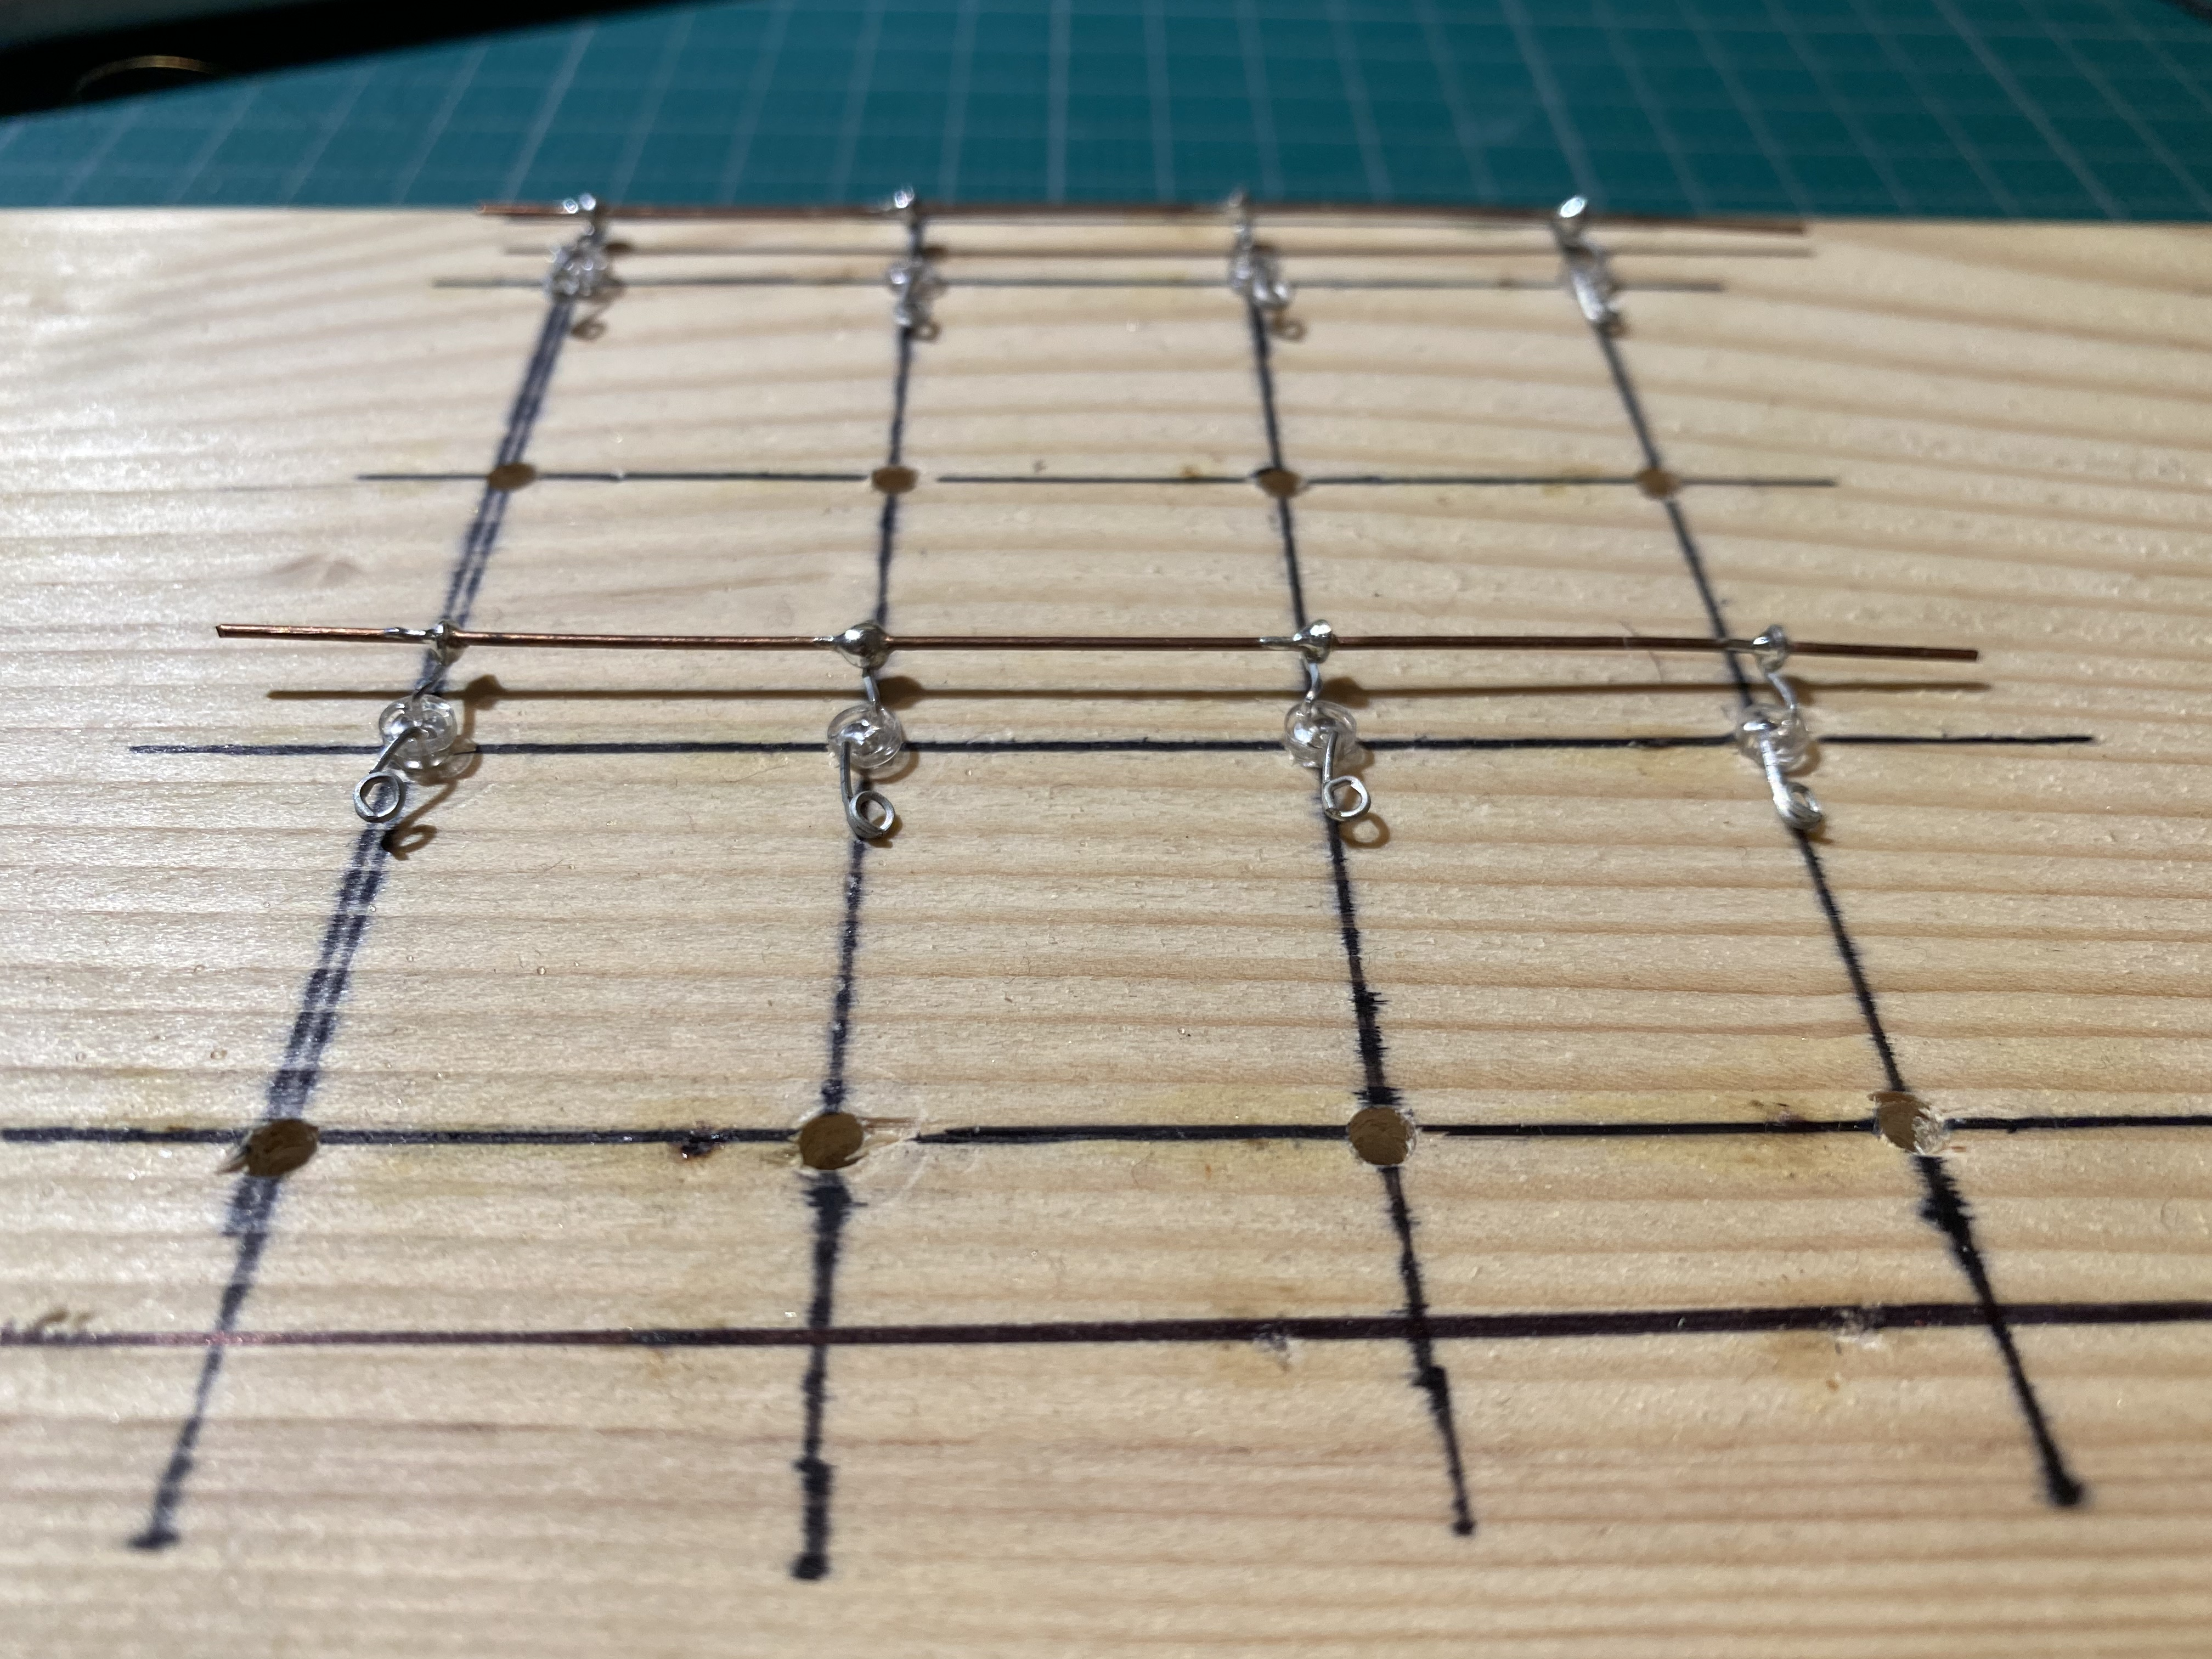
\includegraphics[width=0.42\textwidth]{bilder/jig2.jpeg}
\caption{Jig für die Layers}
\label{fig:jig2}
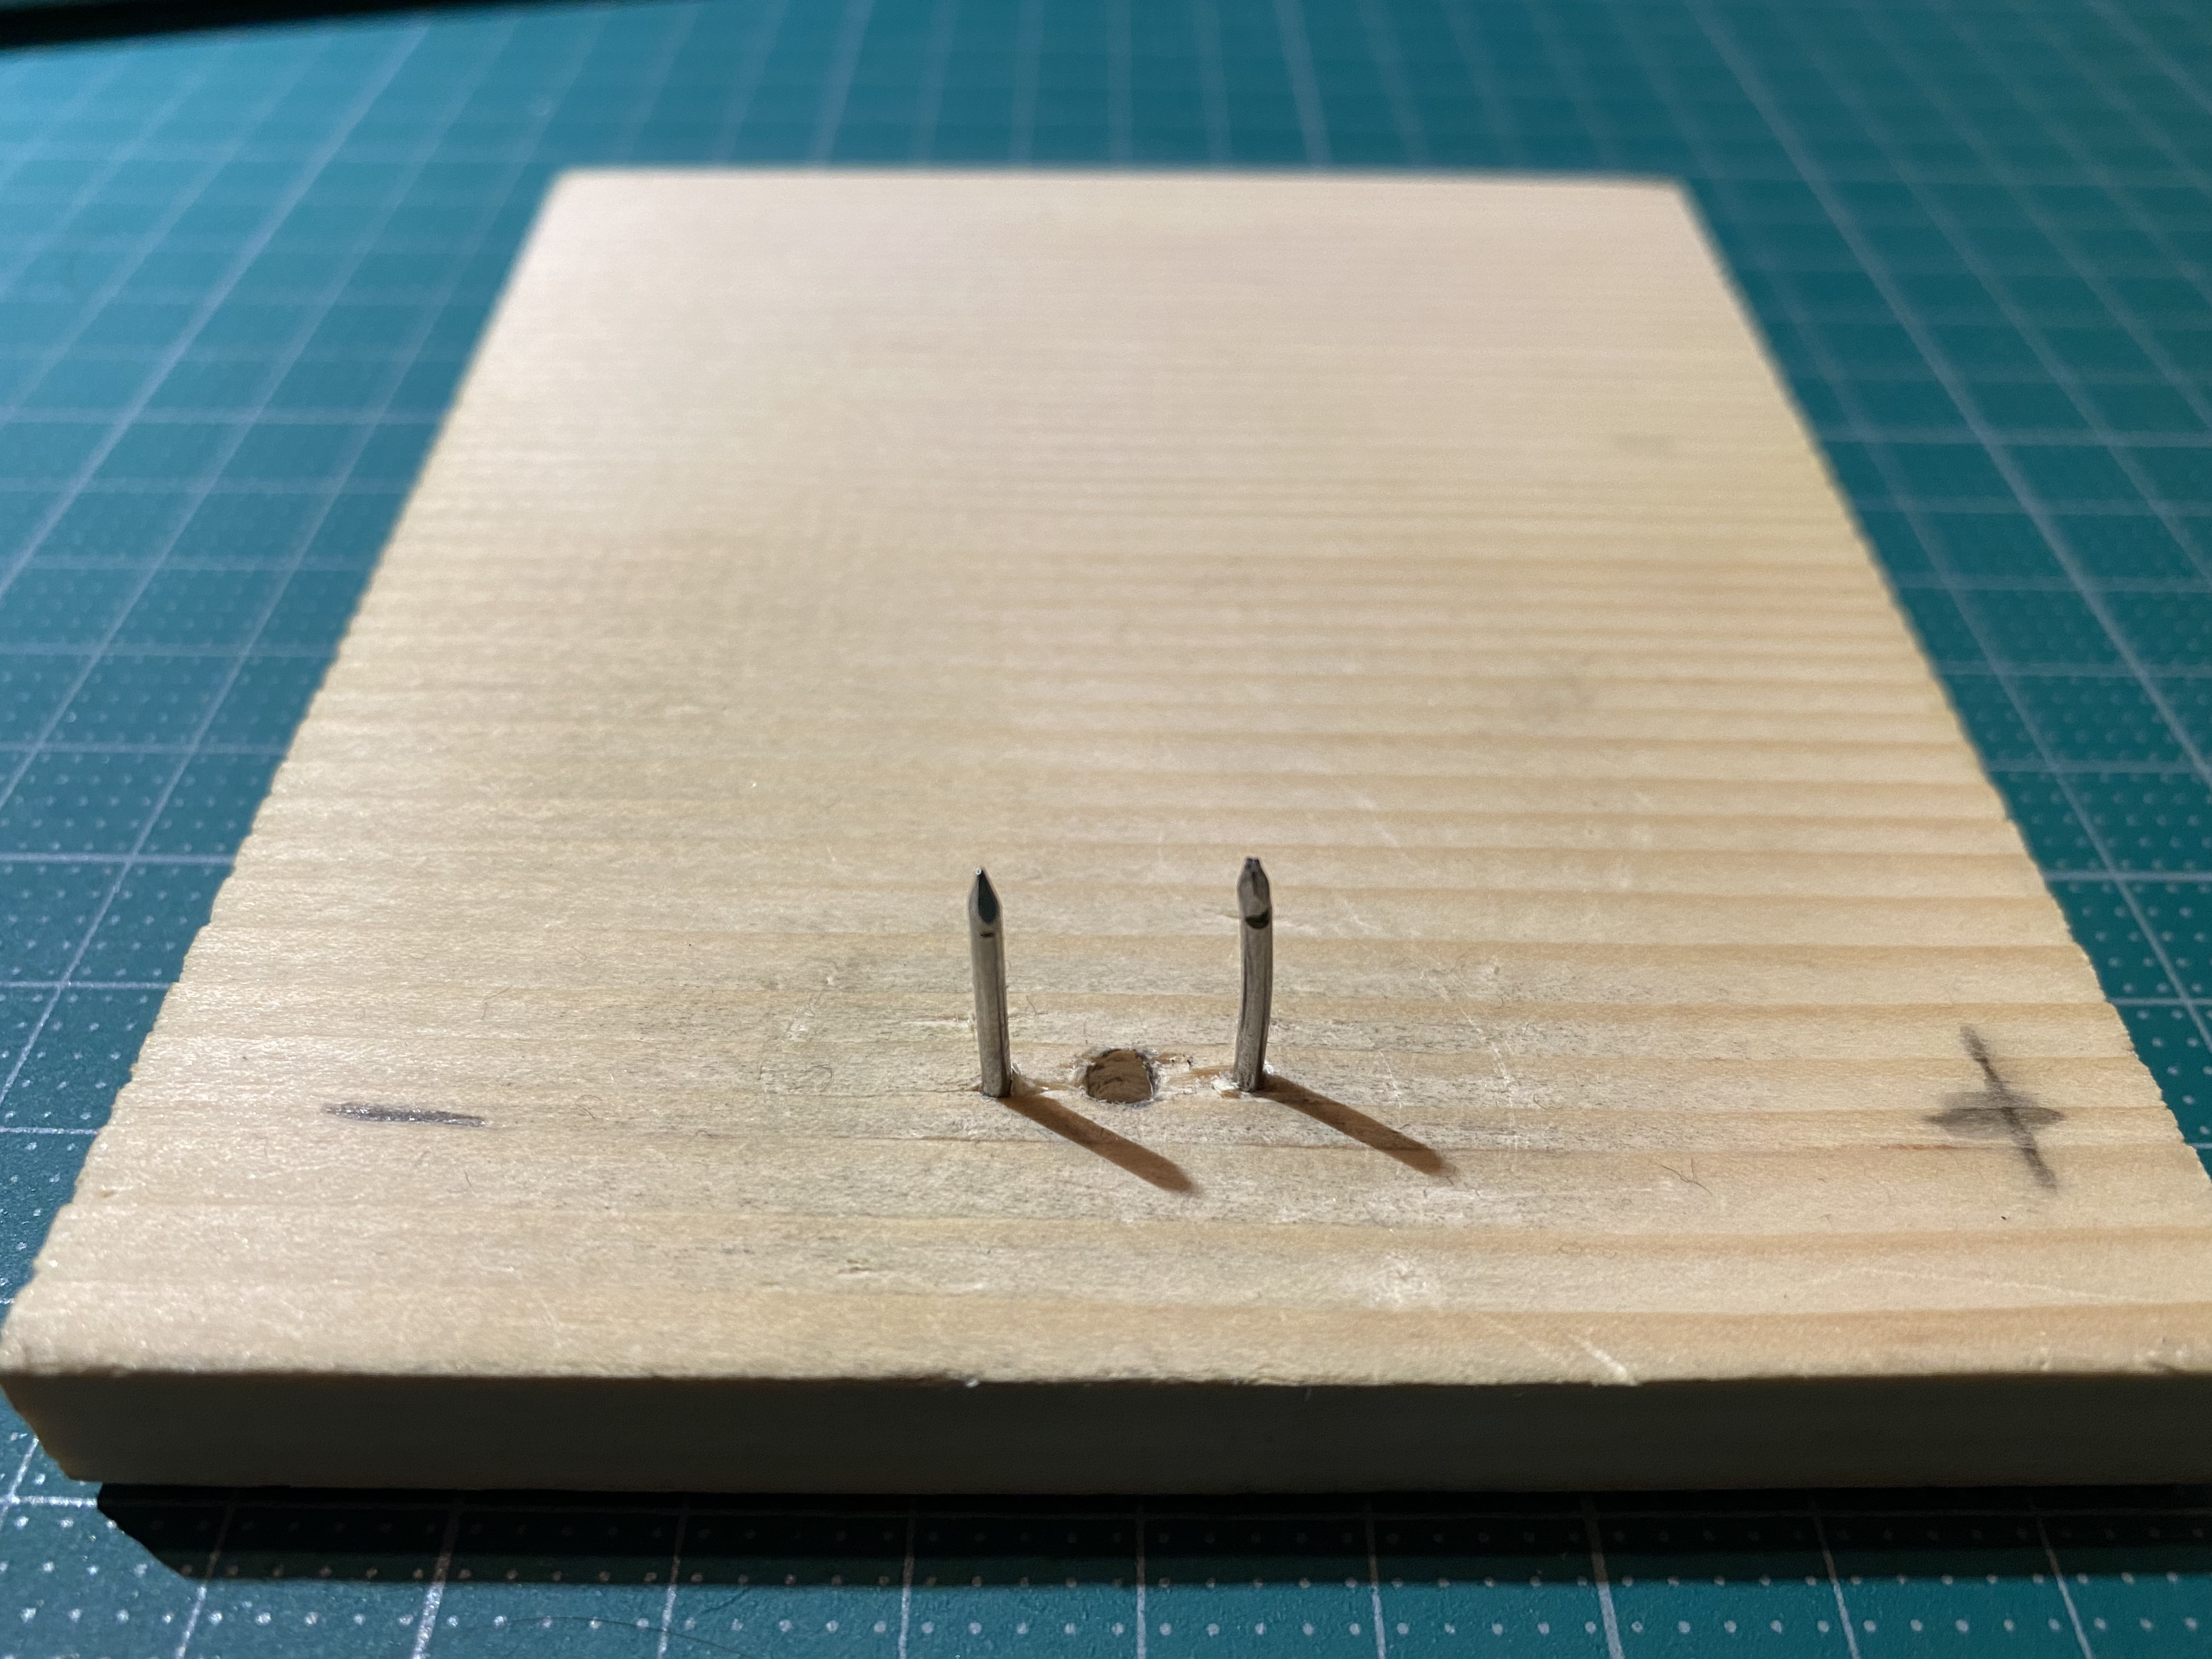
\includegraphics[width=0.42\textwidth]{bilder/jig1.jpeg}
\caption{Jig für die LEDs}
\label{fig:jig1}
\end{center}
\end{figure}

\noindent Die folgenden Werkzeuge wurden für die Kommunikation und als Austausch verwendet.
\begin{itemize}
\item GitHub, sorgte für einen reibungslosen Austausch.
\item WhatsApp, auf welchem die Meetings festgelegt wurden.
\item Zoom, für Onlinemeetings, falls jemand nicht anwesend war.
\item \LaTeX \text{ }für die Dokumentenerfassung.
\end{itemize} 
\section{Sammeln der Daten}
Bevor das Projekt begann, wurde für die Sicherstellung des Projektes der Sensor anhand des Serialports ausgelesen. Mittels Python Programmen wurde die Raumtemperatur gesammelt und geplotet. Genauere Aufbauinformationen findet man im Dokument:\textbf{ Aufbau.pdf}. Das Dokument befindet sich auf dem angegebenen GitHub Repository: \url{https://github.com/ugurtu/CatcProject/blob/main/Aufbau\%20DHT\%2C\%20Programme\%20und\%20Daten/Aufbau.pdf}.\\ Den spezfischen Python Code findet man unter: \url{https://github.com/ugurtu/CatcProject/tree/main/SerialPort_python}
\\ Diesem Dokument aber liegen sowohl der Aufbau des Sensors und auch das Pythonprogramm bei. Wenn man Lüftet, sollte der Sensor in einer bestimmten Zeit eine Reaktion zeigen. Diese Reaktion verhaltet sich in Form von einem entsprechend angehenden LED Lämpchen. Dieses Testen und auslesen des Sensors diente für uns als Sicherstellung. Somit wurde uns klar, dass wir einen funktionstüchtigen Sensor besitzen, welchen wir für dieses Projekt ohne Probleme verwenden konnten.
\begin{figure}[!h]
\begin{center}
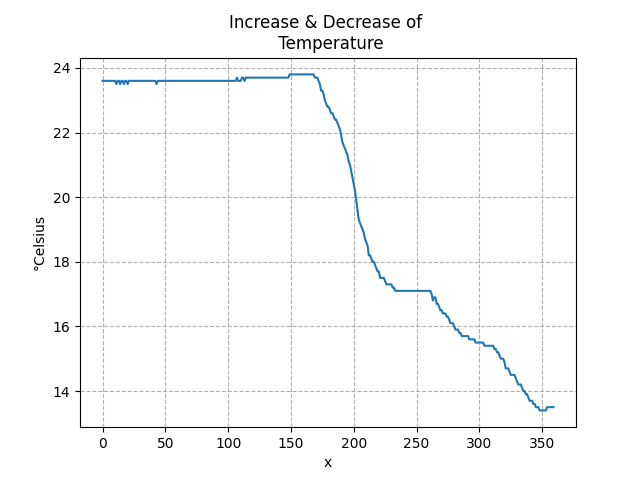
\includegraphics[width=0.49\textwidth]{plot.png}
\caption{Plot des Temperatur Anstiegs und der Abfall}
\label{fig:decrease}
\end{center}
\end{figure}
\begin{figure}[!h]
\begin{center}
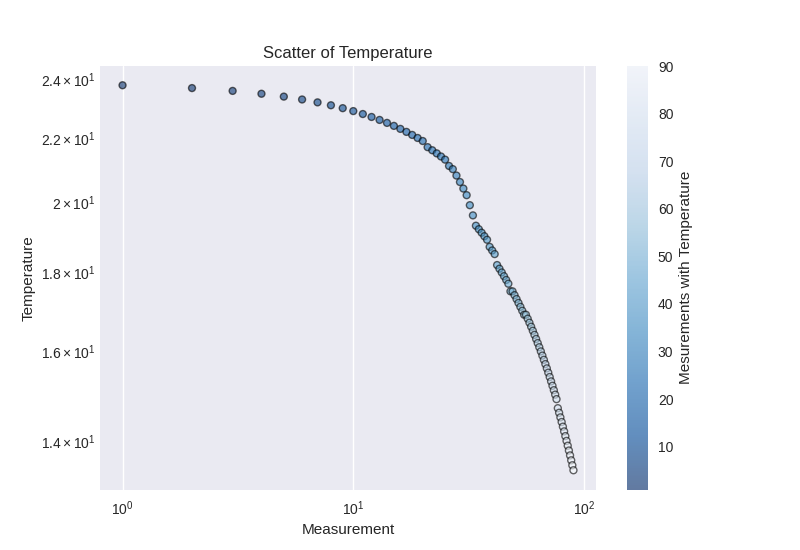
\includegraphics[width=0.53\textwidth]{scatter.png}
\caption{Scatter Plot des Temperatur Abfalls}
\label{fig:scatter}
\end{center}
\end{figure}
\vfill
\begin{figure}[!h]
\begin{center}
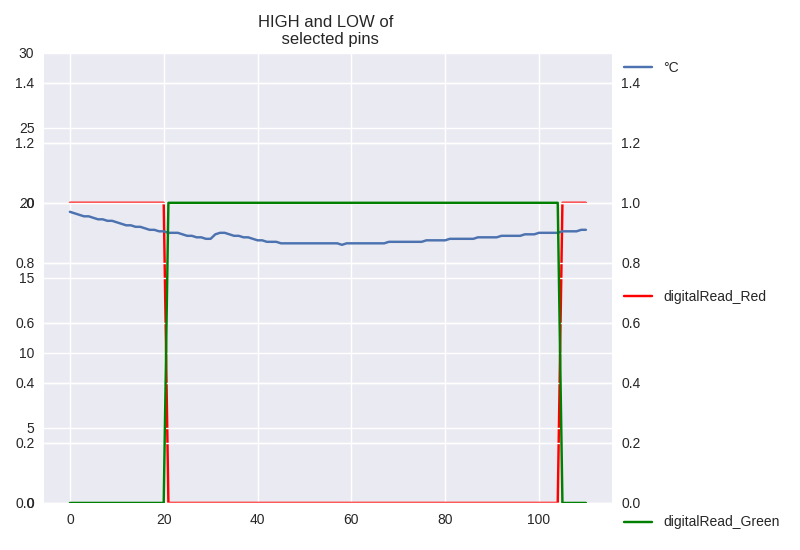
\includegraphics[width=0.49\textwidth]{digitalRead.png}
\caption{HIGH und LOW in einem ersten Test}
\label{fig:highlow}
\end{center}
\end{figure}
\newpage
\subsection{Erkenntnisse durch die Daten}
In der Abbildung \ref{fig:decrease} und \ref{fig:scatter} sieht man wie sich die Temperatur bei offenem Fenster zunehmend verringert. Somit hatten wir Gewissheit, dass der Sensor relativ schnell reagiert und für unser Projekt verwendbar ist. Die x - Achse in der Abbildung \ref{fig:decrease} ist die Zeit. Die Abbildung \ref{fig:scatter} ist Mesurement als 100 Messpunkte definiert. Alle doppelten Daten aus Abbildung \ref{fig:decrease} wurden ignoriert. In der Abbildung \ref{fig:highlow} sollen die zwei Farben, grün und rot, die Farben unserer LED’s und den Zustand HIGH and LOW repräsentieren. Sobald die Temperatur unter 18$^\circ$ C betrug, schalteten sich die grünen LED’s an (HIGH) und die roten LED’s aus (LOW). Damit wurde angezeigt, dass die Bedingung für das Einschlafen optimal ist. Sobald das Fenster wieder geschlossen und die Raumtemperatur damit wieder zugenommen hat, schalteten sich die grünen LED’s aus (LOW) und die roten LED’s gingen wieder an (HIGH).

\section{Umsetzung}
Unser Projekt hat in mehrheitlich sechs Phasen stattgefunden. Diese waren:
\begin{enumerate}[label=(\roman*)]
\item Einkauf
\item Prototyp auf Tinkercad
\item Einzelne Layers verlöten mit LEDs
\item Layers zu einem Cube verlöten
\item Cube mit Arduino verbinden
\item Case
\end{enumerate}
\textbf{Erster Punkt} Wir haben einige Sachen bewusst doppelt gekauft. Falls etwas defekt gewesen wäre, hätten wir keine Zeitengpässe gehabt. \\ \\ 
\textbf{Zweiter Punkt} Dieses folgende umgesetzte \glqq Circuit-Modell\grqq \text{ }wurde von der Grundstruktur so übernommen, allerdings soll angemerkt werden, dass dieses Modell mit einem Arudino UNO erstellt wurde, da kein Arduino ATMega auf Tinkercad zur Verfügung stand. Siehe: Abbildung \ref{fig:tinkercad}
\begin{figure}[h!]
\begin{center}
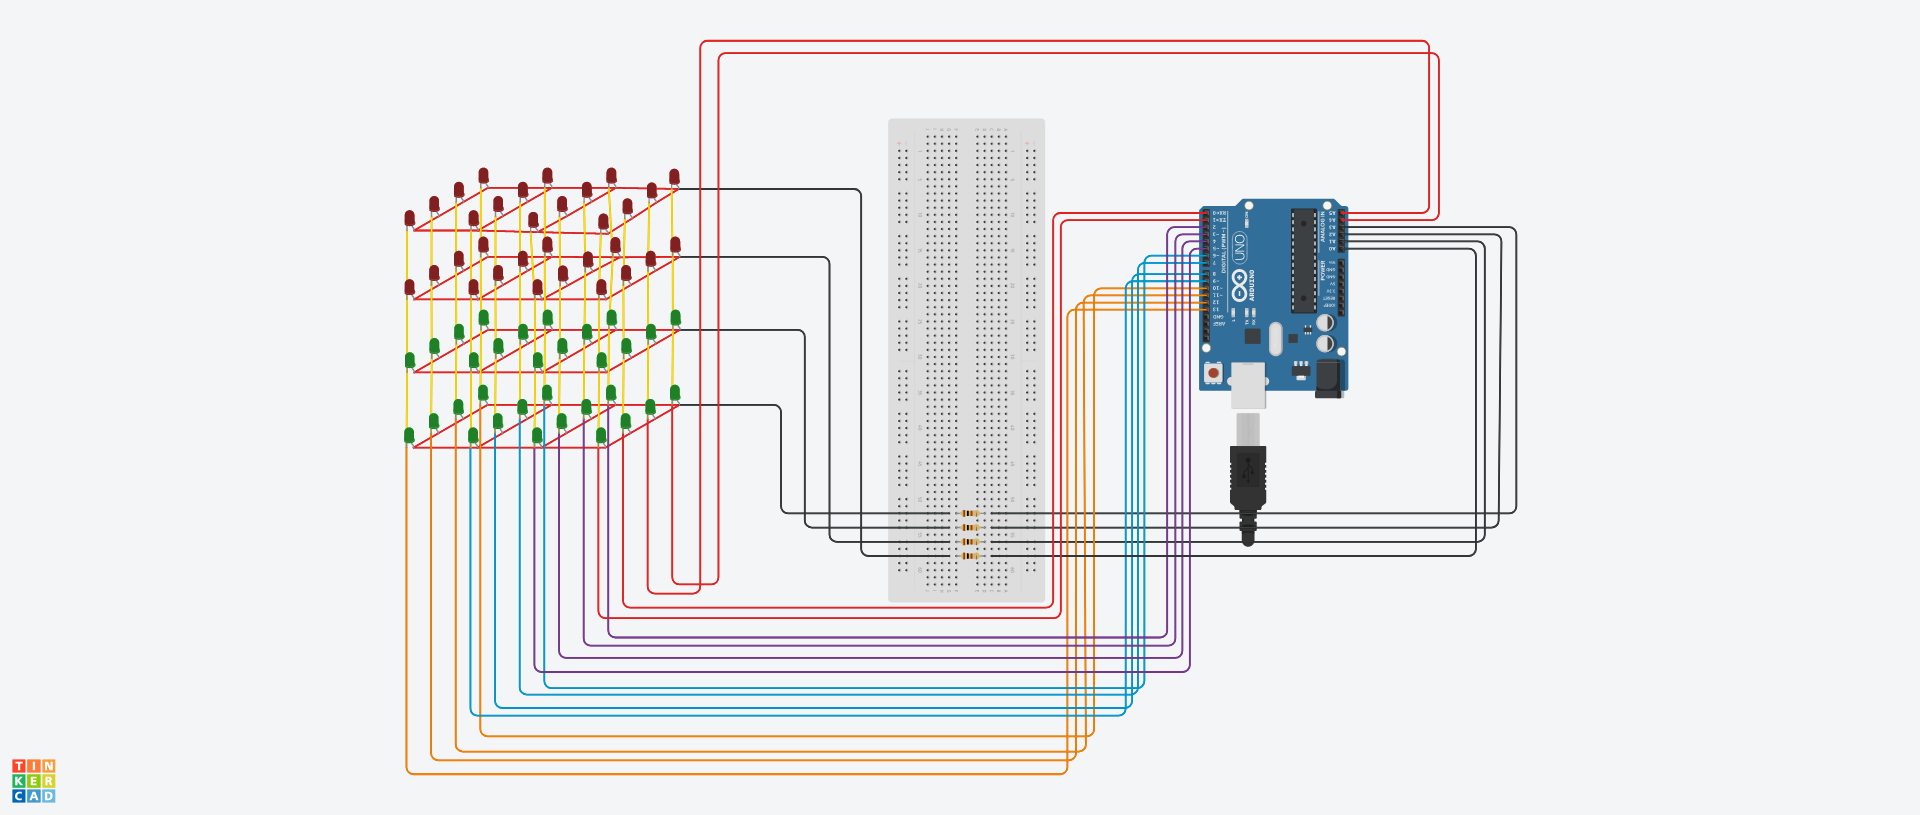
\includegraphics[width=0.53\textwidth]{bilder/ledcube.png}
\caption{LED Cube Circuit mit einem Arduino UNO}
\label{fig:tinkercad}
\end{center}
\end{figure}
\\ \\
\textbf{Dritter Punkt} Die Layers, welche in der Abbildung 7 zu sehen sind leiten den Strom. Es gibt vier davon. 
\begin{figure}[!h]
\begin{center}
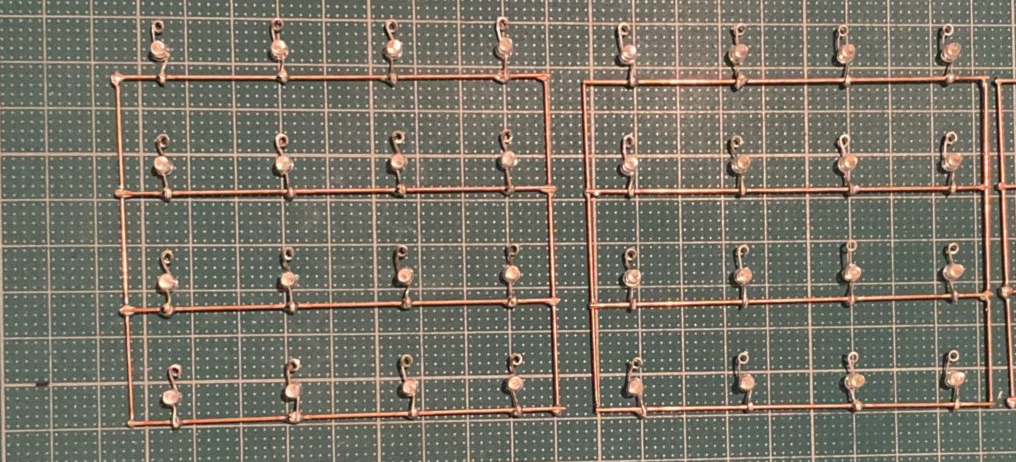
\includegraphics[width=0.53\textwidth]{bilder/layers.jpeg}
\label{fig:anode}
\caption{Anode mit dem Kupferdraht verlötet, zu sehen zwei Layers}
\end{center}
\end{figure}
\\ \\
\textbf{Vierter Punkt} Die Layers, werden durch vertikale Kupferdrähte miteinander verbunden, dies sorgt dafür dass die Kathode verbunden ist. Danach wurde der Cube mit der Europlatine verlötet. Damit jede Ebene, durch den Mikrocontroller Strom bekommt, wurden zusätzlich vier Kupferdrähte jeweils treppenförmig mit den vier Layers verbunden. Jeder Layer ist jeweils mit einem 100 $\Omega$ Widerstand verlötet. Das Datasheet für die LEDs sieht ein Peak Forward Current von 60 mA vor. Daher wurden 100 $\Omega$ verwendet.\footnote{\url{https://www.reichelt.com/de/en/led-3-mm-leaded-green-125-mcd-25--evl-1224-10sygc-p230786.html}} \begin{align}
U = R \cdot I \\
U \coloneqq 5 V, I \coloneqq 0.060 A \\
\frac{5V}{0.060A} = 83.333 \Omega \\
\approx 100 \Omega
\end{align}
Danach wurde auf der linken Seite des sensor Cubes der DHT-22 verlötet. Als letzter Schritt wurden die Kuperdrähte der Kathode und die Pins des Sensors mit Kabeln verlötet, isoliert und mit den Stiftleisten verlötet. Siehe Abbildung \ref{fig:kathode}. 
\begin{figure}[!h]
\begin{center}
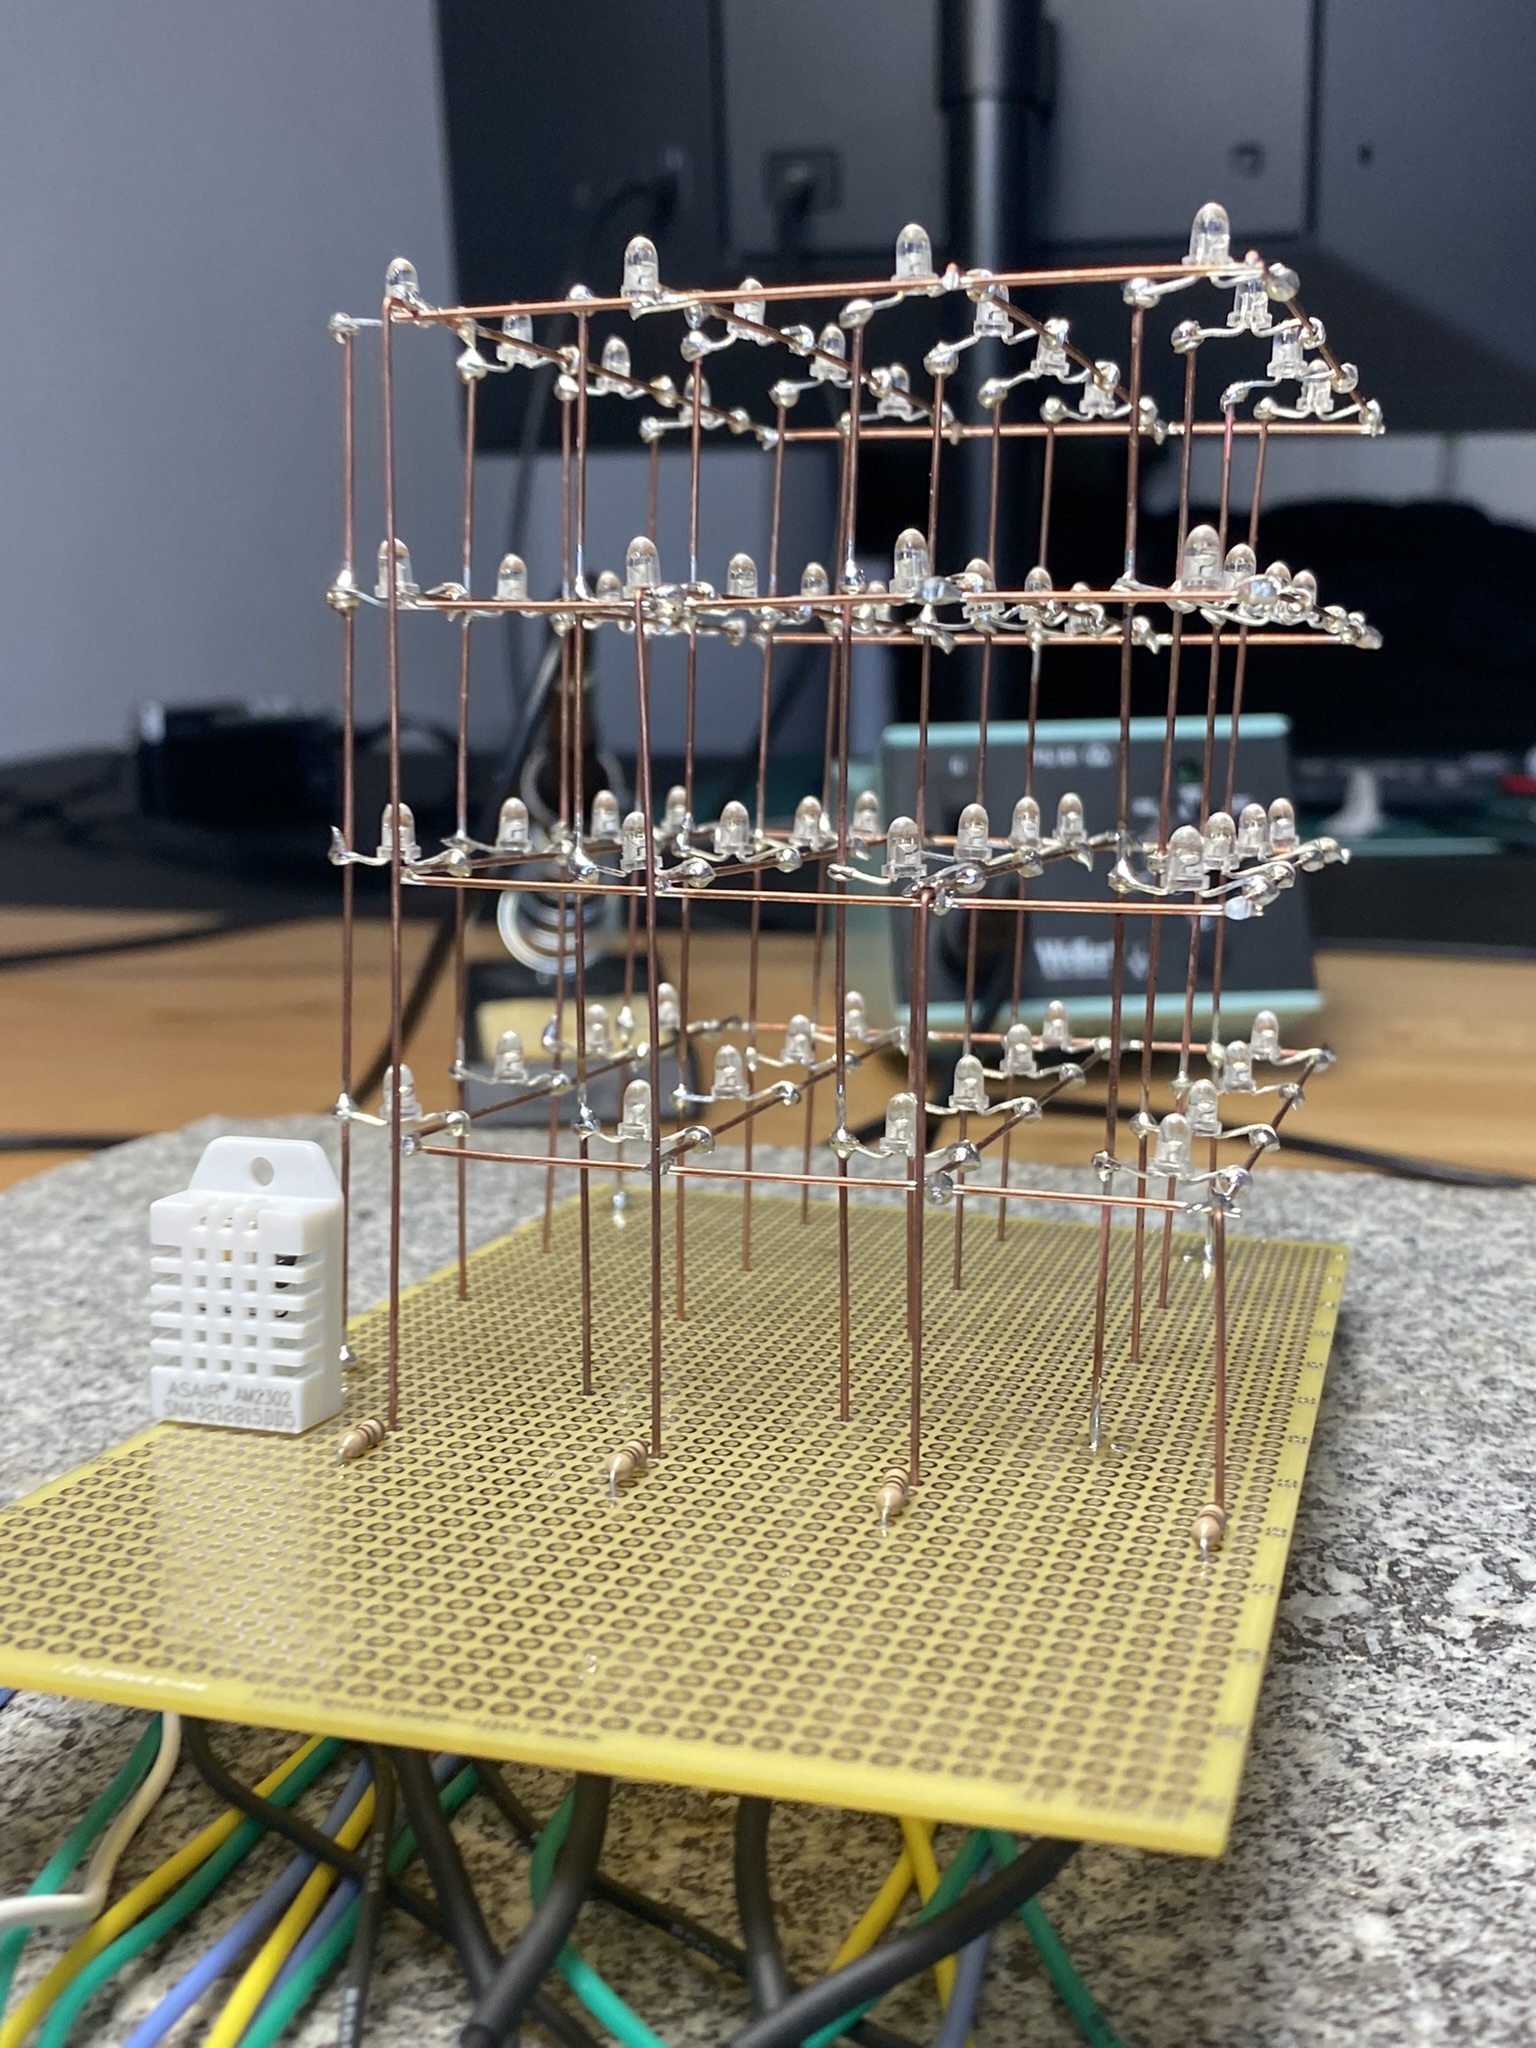
\includegraphics[width=0.42\textwidth]{bilder/cube.jpeg}
\caption{sensor Cube gelötet}
\label{fig:kathode}
\end{center}
\end{figure}\newpage
\noindent \textbf{Fünfter Punkt}
Der 5 Schritt war die entscheidende Phase, da alles fertig war wurden die Pins verbunden. hier eine Übersicht:
\begin{enumerate}
\item A0 $\rightarrow$ versorgt Layer 0 mit Strom.
\item A1 $\rightarrow$ versorgt Layer 1 mit Strom.
\item A2 $\rightarrow$ versorgt Layer 2 mit Strom.
\item A3 $\rightarrow$ versorgt Layer 3 mit Strom.
\end{enumerate}
\textbf{DHT-22 Pins}
\begin{enumerate}
\item DHT-22 Anode $\rightarrow$ 5V.
\item DHT-22 Kathode $\rightarrow$ GND.
\item DHT-22 Digital-Pin $\rightarrow$ 50.
\end{enumerate}
Die Kathode der LEDs sind wie in Abbildung \ref{fig:kathodepins} aufgeteilt. Die Pins werden durch jeweils zwei For-Loops als OUTPUT initialisiert. Einmal für die Layers und einmal für die \glqq Spalten\grqq. Dies hat den Vorteil, dass wir nun durch dieses System jede LED einzeln ansteuern.
\tikzset{darkstyle/.style={circle,draw,fill=gray!40}}
\begin{figure}[hbt!]
\centering
\begin{tikzpicture}
\begin{scope}[every node/.style={circle,thick,draw,fill=gray!40,level distance=200mm,}]
    \node (D48) at (0,0) {D48};
    \node (D46) at (2,0) {D46};
    \node (D44) at (4,0) {D44};
    \node (D42) at (6,0) {D42};
    
    \node (D46) at (2,0) {D46};
    \node (D44) at (4,0) {D44};
    \node (D42) at (6,0) {D42};
    
    \node (D40) at (0,-2) {D40};
    \node (D38) at (2,-2)  {D38};
    \node (D36) at (4,-2) {D36};
    \node (D34) at (6,-2) {D34};
    
    \node (D32) at (0,-4) {D32};
    \node (D30) at (2,-4)  {D30};
    \node (D28) at (4,-4) {D28};
    \node (D26) at (6,-4) {D26};
    
    \node (D24) at (0,-6) {D24};
    \node (D22) at (2,-6)  {D22};
    \node (A5) at (4,-6) {A5};
    \node (A4) at (6,-6) {A4};
    
\end{scope}

\begin{scope}[>={Stealth[black]},
              every node/.style={fill=gray!40,circle,thick},
              every edge/.style={draw=red,very thick}]
     \draw [color=red!100,->,line width=1] (A4) -- (A5);
     \draw [color=red!100,->,line width=1] (A5) -- (D22);
     \draw [color=red!100,->,line width=1] (D22) -- (D24);
     \draw [color=red!100,->,line width=1] (D24) -- (D32);
     \draw [color=red!100,->,line width=1] (D32) -- (D40);
     \draw [color=red!100,->,line width=1] (D40) -- (D48);
     
     \draw [color=red!100,->,line width=1] (D48) -- (D46);
     
     \draw [color=red!100,->,line width=1] (D46) -- (D38);
     \draw [color=red!100,->,line width=1] (D38) -- (D30);
     \draw [color=red!100,->,line width=1] (D30) -- (D22);
     
     \draw [color=red!100,->,line width=1] (D46) -- (D44);
     \draw [color=red!100,<-,line width=1] (D44) -- (D36);
     \draw [color=red!100,<-,line width=1] (D36) -- (D28);
     \draw [color=red!100,<-,line width=1] (D28) -- (A5);
     
     \draw [color=red!100,->,line width=1] (D44) -- (D42);
     \draw [color=red!100,->,line width=1] (D42) -- (D34);
     \draw [color=red!100,->,line width=1] (D34) -- (D26);
     \draw [color=red!100,->,line width=1] (D26) -- (A4);
   
\end{scope}
\end{tikzpicture}
\caption{Obere Ansicht des sensor Cubes mit den Verbundenen Pins und des Stromflusses}
\label{fig:kathodepins}
\end{figure} \\ \\
\textbf{Sechster Punkt} Als der sensor Cube fertig war und wir somit wussten, dass wir das Ziel erreicht haben, haben wir uns auf die Suche nach einem passenden Case gemacht. In einem Meeting wurde die Entscheidung getroffen, ein Case aus Plexiglas herzustellen. In verschiedenen Geschäften suchte man das passende Plexiglas, nach Scharnieren und Klebstoffen. Das Plexiglas wurde mit den passenden Massen geschnitten und schlussendlich zu einem Rechteck zusammengeklebt. Anschliessend wurden in die Seite des Case, sowie in die Europlatine zwei Schaniere montiert. Dies sollte uns ermöglichen, einen Türähnlichen Mechanismus zu haben. sind die Kabel und das Arduino in Sicherheit. Ausserdem wurde ein Loch in die Seite des Case gefräst, um die Stromversorgung zu gewährleisten Ebenfalls können Reparaturen vorgenommen werden, falls ein Kabel defekt ist. Für das Ergebnis siehe Abbildung \ref{fig:cubewcase}.
\begin{figure}[!h]
\begin{center}
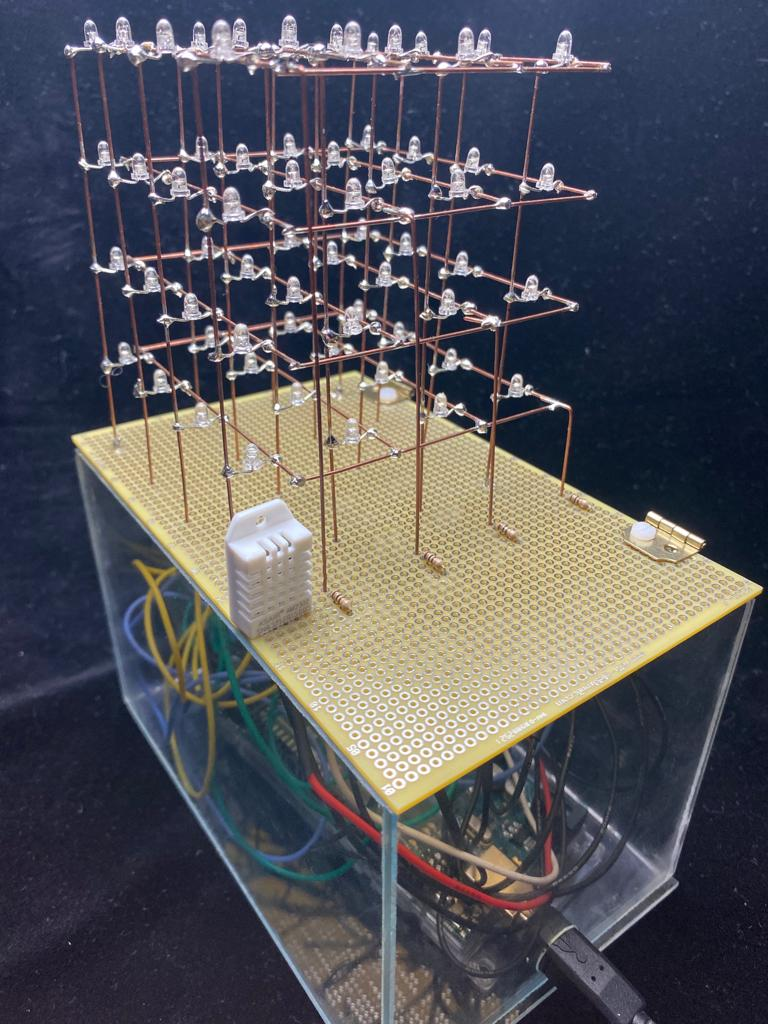
\includegraphics[width=0.42\textwidth]{bilder/cubewcase.jpeg}
\caption{Cube mit Case}
\label{fig:cubewcase}
\end{center}
\end{figure}
\newpage
\section{Resultat}
\label{section:result}
Der Cube ist unserer Meinung nach genau und symmetrisch gelötet. Auch wenn es noch Raum nach oben gibt, sind wir mit dem Endprodukt sehr zufrieden. Zudem lässt das durchsichtige Case einen direkten Blick auf das Innenleben des Cubes zu. Da für die Verdrahtung sehr wenig Platz war, haben wir Schrumpfschläuche an den Enden
der Kabel benutzt. Diese verhindern einen allfälligen Kurzschluss. Danach hatten wir zwischen dem Arduino und allen LEDs sowie dem Sensor eine sichere Verbindung. In Abhängigkeit von den Messdaten kann der Cube die folgenden fünf Muster wiedergeben:

\begin{itemize}
\item Temperatur: $<$ 15$^\circ$ C Raumtemperatur
\begin{itemize}
\item[$\square$] Dynamisches/pulsierendes Feedback
\end{itemize}
\item Temperatur: $\geq$ 15$^\circ$ C Raumtemperatur $\leq$ 18$^\circ$ C
\begin{itemize}
\item[$\square$] Feuchtigkeit: $<$ 30 \% Luftfeuchtigkeit im Raum
\begin{itemize}[label=$\ast$]
\item Dynamisches Regenmuster von unten nach oben 
\end{itemize}
\end{itemize}
\begin{itemize}
\item[$\square$] Feuchtigkeit: $\geq$ 30 Luftfeuchtigkeit im Raum $ \leq$ 60  \%
\begin{itemize}[label=$\ast$]
\item Die zwei grünen Levels leuchten statisch
\end{itemize}
\end{itemize}
\begin{itemize}
\item[$\square$] Feuchtigkeit: $>$ 60 \% Luftfeuchtigkeit im Raum
\begin{itemize}[label=$\ast$]
\item Dynamisches Regenmuster von oben nach unten
\end{itemize}
\end{itemize}
\item Temperatur: $> $ 18$^\circ$ C Raumtemperatur
\begin{itemize}
\item[$\square$] Dynamisches/ propellerartiges Leuchtmuster
\end{itemize}
\end{itemize}
Durch die visuelle Wiedergabe der LEDs hat man Zeitnah ein Feedback über das Raumklima. Die dynamischen Leuchtmuster lassen sich schnell interpretieren und es kann entsprechend reagiert werden. Nach Anpassungen des Raumklimas leuchtet das statische Muster in grün. Danach steht einer guten Einschlafphase \glqq nichts\grqq \text{ }mehr im Weg.

\section{Gewonnene Erkentnisse}
Dieser Abschnitt besteht nicht nur aus einer Erkenntnis sondern aus mehreren Erkenntnissen. Deshalb sollen in den nachfolgenden Abschnitten folgende Erkentnisse angesprochen werden: 
\begin{enumerate}
\item Die Fähigkeit beziehungsweise die Nützlichkeit des sensor Cubes im Alltag,
\item Erkenntnisse über das verwendete Material,
\item Zeitmanagement bis zur Abgabe,
\item Verbesserungen für ein nächstes Projekt.
\end{enumerate}

\subsection{Nützlichkeit im Alltag}
Das unser Cube im Stande ist auf unterschiedlichliche Temperaturen und eine veränderte Luftfeuchtigkeit zu reagieren ist ausser Frage. Dies wurde in einem Praxistest bei allen drei Gruppenmitgliedern zu Hause getestet. Das bei einer spezifischen Luftfeuchtigkeit \& Temperatur spezifische festgelegte Muster als Feedback angezeigt werden sollen ist vorhanden. \newline Wir sind per E-Mail mit Schlafprofessor Prof. Dr. Björn Rasch in Kontakt getreten, um zusätzliche Informationen über die optimale Schlaftemperatur und Luftfeuchtigkeit zu erhalten. Aus einer E-Mail von 03.01.22 wurden drei Punkte deutlich. 
\begin{enumerate}
\item Der Schlaf steht in Korrelation mit der psychologischen Verfassung des Benutzers des Kubus.
\item Die Temperatur für den optimalen Schlaf hängt von dem Microklima unter der Bettdecke ab.
\item Verschiedene Studien kommen zum Schluss, dass 30-50\% oder 30-60\% Luftfeuchtigkeit optimal sind.    
\end{enumerate}
\textbf{Zu Punkt eins} soll keine Stellung genommen werden, da wir über keine fundierte psychologische Ausbildung verfügen, selbst wenn das der Fall wäre, würde dies den Rahmen des Reports sprengen. \\ \\ \textbf{Zu Punkt zwei} sind wir der gleichen Meinung, dass wenn eine Bettdecke zu warm gibt, dies sich auf das Einschlafen negativ auswirkt. Trotzdem hat der Cube das Einschlafen bei allen Gruppenmitgliedern positiv beeinflusst. Somit sehen wir einen direkten Zusammenhang zwischen dem Raumklima und der Qualität des Einschlafens. Wir vermuten, dass durch die zusätzliche Wahl einer passenden Bettdecke die Qualität des Einschlafens weiter verbessert wird. \\ \\ \textbf{Zu Punkt drei}, dass die Luftfeuchtigkeit stimmen muss für den Schlaf/Einschlaf, vorallem in einer kalten Jahreszeit, da kalte Luft relativ trocken ist, kann unser Kubus auch evaluieren. \\ \\
\textbf{Fazit} Die Benutzung des sensor Cubes kann hilfreich sein beim Einschlafen. Allen drei Gruppenmitgliedern hat der sensor Cube geholfen. 
 
\subsection{Das verwendete Material} 
Folgende Komponenten wurden verwendet: 
\begin{enumerate}
\item Kupferdraht
\item Kabel mit einer Litze
\item Arduino UNO 328P $\rightarrow$ Arduino ATMega 2560
\item Lötzinn
\item Flussmittel
\item Schrumpfschlauch
\item Euro-Platine aus Epoxidharz
\item Plexiglas
\item Löt-Station
\item DHT-22
\item LEDs
\item Scharniere
\item Sekundenkleber
\item USB-Stecker - Typ B
\item Multimeter
\item Heissluftföhn
\item Bohrmaschine
\end{enumerate}
In der Tabelle \ref{table:problems} auf der nächsten Seite sollen nur die Teile aufgelistet werden, welche Probleme bereitet haben. Die Komponenten die nicht in der Tabelle sind, haben \textbf{keine} Probleme verursacht.
\begin{table}
    %% \centering % not needed
    \caption{Probleme und Lösungen}
    \rowcolors{1}{}{Gray}
    \begin{tabular}{p{\mylength}|p{\mylength}|p{\mylength}}
        \hline
        \textbf{Komponente} & \textbf{Problem}  &\textbf{Lösung}  \\
        \hline \hline
        Kupferdraht & Der Kupferdraht, welcher bestellt wurde, war beschichtet und ohne Lötzinn war dieser nicht Leitfähig. Die Schicht musste geschmolzen werden oder abgeschliffen werden  & Neuer Kupferdraht wurde erworben\\
        Arduino     & Da wir alle LEDs einzeln ansteuern wollten aber auch den Sensor verbauen mussten, waren wir gezwungen mit i$^2$c zu arbeiten oder mehr Pins haben& Ugur entschied sich im Sinne der Gruppe auf einen Arduino ATMega 2560 umzustellen        \\
        Lötzinn        & Der Lötzinn welcher mitgegeben wurde, war relativ alt und ergab beim ersten Löten Zinnkugeln, welche optisch nicht ansprechend waren & Flussmitttel wurde erworben \\
        Schrumpfschlauch         & Der Schrumpfschlauch der erworben wurde, hatte einen zu kleinen Durchmesser für die Verbingdungskabel &  Schrumpfschlauch mit 3mm, welcher auf eine grösse von 1mm schrumpfte wurde erworben\\
        Euro-Platine aus Epoxidharz   & Bis heute sind wir in der Gruppe nicht einig, ob wir die Euro-Platine anders herum hätten verwenden sollen, da der Lötzinn nicht haftete & -      \\
        Plexiglas   & Wir wollten nicht nur ein Platz für unseren Arduino, sondern auch ein Case für den Cube aus Plexiglas, leider reflektierte das Material die Lichter der LEDs zu stark. Somit war nicht eindeutig erkennbar, welche LED rot oder Grün leuchtete. & Verzicht den Cube in ein Plexiglas gehäuse zu stellen.      \\
        Löt-Station & Die Spitze des Lötkolbens, welcher zur Verfügung gestellt wurde, war oxidiert. Somit war es nicht möglich mit dieser Löt-Station zu löten, entweder musste die Lötspitze gereinigt werden oder eine andere Lötstation musste her. & Ugurs Arbeitgeber verlieh eine professionelle Löt-Station aus.\\
        DHT-22   & Ein Sensor der mitgeliefirt wurde, war defekt. Da wir aber aus Sicherheitsgründen zwei bestellt haben, hatten wir ein Backup & Der zusätzliche Sensor wurde verwendet.      \\
        Sekundenkleber & Die Kombination aus Sekundenkleber und Plexiglas verträgt sich nicht gut. Beim ausprobieren hat Berkan festgestellt das Spuren des Klebers sichtbar werden & Berkan hat trotz der Einschränkung, versucht so sauber wie möglich zu arbeiten\\
        USB-Stecker - Typ B & Der USB-Stecker Typ B war relativ dick. Da wir keine Werkstatt haben, standen uns nur wenige Aufsätze zur Verfügung. Das Loch, welcher für das Kabel gedacht ist, ist ein bisschen Eng. & -  \\
        
        \hline
    \end{tabular}
    \label{table:problems}
\end{table}
\newpage
\subsection{Zeitmangement}
Da wir einen strikten Gantt-Chart befolgt haben, wurde alles nach Zeitplan erledigt. Wir waren mit dem sensor Cube am 31. Dezember 2021 fertig. Somit konnten wir viel testen und uns zusätzliche Gedanken darüber machen, wie wir die Luftfeuchtigkeit zusätzlich in unser Projekt integrieren können. Ausserdem hatten wir genug Zeit um Ästhetische Aspekte, wie die LED Feedbacks und das Case fertigzustellen. Wir können behaupten, dass wir die Verwendung des Gantt-Charts nochmal in einem ähnlichen Projekt einbinden würden, da dieses den Zeitplan relativ gut eingeteilt hat und wir somit immer wieder überprüfen konnten, wo wir stehen.  
\subsection{Verbesserungswürdig}
Wir kamen zum Entschluss, dass wir in einem nächsten Projekt mehr Zeit für die Planung investieren würden. Diese zusätzliche Zeit hätte uns viel Mühe und Zeit erspart. Viele Erkentnisse kamen zu spät, beispielsweise haben wir das Kupfergestell gelötet ohne zu überlegen, wie wir es in die Euro-Platine reinbekommen sollen. Dieses Problem wäre einfacher zu lösen gewesen, wenn wir das Grundgerüst direkt in die Europlatine integriert hätten. Das gleiche Problem hatten wir auch mit unserem Case, welches sich schwerer als gedacht erwies, da wir schon ein fertigen Kubus hatten welchen wir nun mit einem Case austatten wollten. Zudem ist es auch wichtig sich vorher schon Gedanken zu machen ob uns genug Pins zur Verfügung stehen, dass hat uns zwei Tage gekostet, da die Lieferung bisschen verzögert war.
\newpage
\section{Danksagung}
Folgenden Personen/ dem Arbeitgeber soll gedankt werden: \\
\newline \textbf{Frau Sarah-Lia Andrea Wotke}, Sie hat Ugur eine Einführung in das Löten gegeben, er konnte sein Wissen mit Berkan und Silvan teilen. Zu dem hat Sie wichtige Tipps gegeben, wie wir die Kabel isolieren sollten. \newline \newline
\textbf{Herr Prof. Dr. Björn Rasch} an der Universität Fribourg, er hat dem Projekt eine andere Sichtweise gegeben.\newline \newline
\textbf{Herr Ilir Ferati} Welcher wichtige Tipps bezüglich des Gehäusebaus gegeben hat.\newline \newline
Als letztes wollen wir uns bei der \textbf{Abteilung Technik des Telebasels} bedanken. Diese hat uns das nötige Werkzeug zur Verfügung gestellt, welche den Zeitplan sichergestellt haben.

\end{document}
